
\documentclass{article}

\usepackage[T1, T2A]{fontenc}
\usepackage[utf8]{inputenc}
\usepackage[russian]{babel}
\usepackage{amsmath}
\usepackage[left=2cm, right=2cm, top = 2cm, bottom = 2cm, bindingoffset=0cm]{geometry}
\usepackage{indentfirst}
\usepackage{graphicx}
\usepackage{enumerate}

\usepackage{listings}

\graphicspath{{images/}}

\linespread{1.5}

\title{Отчет по анализу алгоритмов}
\date{2020}
\author{Pavel Khetagurov}

\begin{document}
	\begin{table}[ht]
	\centering
	\begin{tabular}{|c|p{400pt}|} 
	\hline
		\begin{tabular}[c]{@{}c@{}} 
\includegraphics[scale=0.15]{EmblemBMSTU} \\\end{tabular} &
		\footnotesize\begin{tabular}[c]{@{}c@{}}\textbf{Министерство~науки~и~высшего~образования~Российской~Федерации}\\\textbf{Федеральное~государственное~бюджетное~образовательное~учреждение}\\\textbf{~высшего~образования}\\\textbf{«Московский~государственный~технический~университет}\\\textbf{имени~Н.Э.~Баумана}\\\textbf{(национальный~исследовательский~университет)»}\\\textbf{(МГТУ~им.~Н.Э.~Баумана)}\\\end{tabular}  \\
	\hline
	\end{tabular}
\end{table}
\noindent\rule{\textwidth}{4pt}
\noindent\rule[14pt]{\textwidth}{1pt}
\hfill 
\noindent
\makebox{ФАКУЛЬТЕТ~}%
\makebox[\textwidth][l]{\underline{~~~~«Информатика и системы управления»~~~~~~~~~~~~~~~~~~~~~~~~~~~~~~~~~~~~~~~~~~~~}}%
\\
\noindent
\makebox{КАФЕДРА~}%
\makebox[\textwidth][l]{\underline{~~~~~~~«Программное обеспечение ЭВМ и информационные технологии»~~~~~~~~}}%
\\


\begin{center}
	\vspace{3cm}
	{\bf\huge Отчёт\par}
	{\bf\Large по лабораторной работе №7\par}
	\vspace{0.5cm}
\end{center}


\noindent
\makebox{\large{\bf Название:}~~~}
\makebox[\textwidth][l]{\large\underline{~Поиск в словаре~~~~~~~~~~~~~}}\\

\noindent
\makebox{\large{\bf Дисциплина:}~~~}
\makebox[\textwidth][l]{\large\underline{~Анализ алгоритмов~~~~~~~~~~~~~~~~~~~~~~~~~~~~~~~~~~~~~~~~~~~~~~~~~~~~}}\\

\vspace{1.5cm}
\noindent
\begin{tabular}{l c c c c c}
    Студент      & ~ИУ7-55Б~               & \hspace{3.5cm} & \hspace{3.5cm}                 & &  Хетагуров П.К \\\cline{2-2}\cline{4-4} \cline{6-6} 
    \hspace{3cm} & {\footnotesize(Группа)} &                & {\footnotesize(Подпись, дата)} & & {\footnotesize(И.О. Фамилия)}
\end{tabular}

\vspace{1cm}

\noindent
\begin{tabular}{l c c c c}
    Преподователь & \hspace{6cm}   & \hspace{3.5cm}                 & & Л.Л. Волкова \\\cline{3-3} \cline{5-5} 
    \hspace{3cm}  &                & {\footnotesize(Подпись, дата)} & & {\footnotesize(И.О. Фамилия)}
\end{tabular}

\begin{center}	
	\vfill
	\large \textit {Москва, 2020}
\end{center}

\thispagestyle {empty}
\pagebreak
	\newpage
	\tableofcontents
	\newpage
	\begin{center}
	    \section*{Введение}
	\end{center}
	\addcontentsline{toc}{section}{Введение}
		\indent \indent В данной лабораторной работе будут рассмотренны и проанализированы такие реализации алгоритма поиска расстояния Левенштейна как:
		\begin{enumerate}
		\item матричная реализация;
		\item рекурсивная без матрицы;
		\item рекурсивная с матрицей;
		\item матричная реализация алгоритма поиска расстояния Дамерау-Левенштейна.
		\end{enumerate}
	\newpage
	\section{Аналитическая часть}
	В данном разделе будут поставлены цели и задачи работы, будут рассмотренны основные теоритические сведения связанные с алгоритмами поиска расстояния Левенштейна и Дамерау-Левенштейна.
		\subsection{Цель и задачи работы}
			\textbf{Цель работы:}
			\newline
			\indent Реализовать и сравнить по эффективности(емкостной, временной разные алгоритмы нахождения расстояния Левенштейна и Дамерау-Левенштейна.
			\newline \indent
			\textbf{Задачи работы:}
			\indent \begin{enumerate}[1)]
				\item дать математическое описание расстояния Левенштейна и Дамерау-Левенштейна;
				\item разработать алгоритмы поиска расстояний;
				\item реализовать построенные алгоритмы;
				\item провести эксперименты по замеру времени работы разработанных алгоритмов;
				\item провести сравнения алгоритмов по затраченному времени и максимальной затраченной памяти;
				\item дать теоритическую оценку затрачиваемой памяти.
			\end{enumerate}
		\subsection{Формула для нахождения расстояния Левенштейна}
		Расстояние Левенштейна (редакционное расстояние) - это минимальное количество редакционных операций, которое необходимо совершить для преобразования одной строки в другую.
		\newline
		\indent Список редакционных операций:
		\begin{itemize}
		\item вставка (I);
		\item удаление (D);
		\item замена (R);
		\item совпадение (M).
		\end{itemize}
		 \indent  \indent	При этом операции I, D, R имеют вес 1, а M - 0.
Пусть есть две строки $s_1$ и $s_2$, индексируемые с 1. Тогда расстояние Левенштейна (L) определяется следующей реккурентной формулой (\ref{levenshtainMath}):
			\begin{equation}\label{levenshtainMath}
			D(s_1[1...i], s_2[1...j]) = 
			\begin{cases}
			   0,  &\text{i = 0, j = 0}\\
			   i, &\text{i > 0, j = 0}\\
			   j, &\text{i = 0, j > 0}\\
			   min(D(s_1[1...i], s_2[i...j - 1]) + 1, \\
	     			    D(s_1[1...i - 1], s_2[i...j - 1]) + \begin{cases}
	     			                           1, &\text{Если $s_1$[i] != $s_2$[j]},\\0, &\text{Иначе}
	     			                           \end{cases} &\text{i > 0, j > 0}\\
			         D(s_1[1...i - 1], s_2[i...j]) + 1)\\
			         \end{cases}
			 \end{equation}, где $s_1$[1...i] и $s_2$[1...j] - строки длинной i и j соответственно.
		\subsection{Формула для нахождения расстояния Дамерау-Левенштейна}
		Расстояние Дамерау-Левенштейна является модификацией расстояния Левенштейна, к возможным редакторским операциям добавляется операция перестановки двух соседних символов (X) со штрафом 1.
		\newline
		\indent Модифицированная формула \ref{levenshtainMath} для нахождения расстояния Дамерау-Левенштейна:
			\begin{equation}\label{damerauLevenshtainMath}
			D(s_1[1...i], s_2[1...j]) = 
			\begin{cases}
			   0,  &\text{i = 0, j = 0}\\
			   i, &\text{i > 0, j = 0}\\
			   j, &\text{i = 0, j > 0}\\
			   min(D(s_1[1...i], s_2[i...j - 1]) + 1, \\
	     			    D(s_1[1...i - 1], s_2[i...j - 1]) + \begin{cases}
	     			                           1, &\text{Если $s_1$[i] != $s_2$[j]},\\0, &\text{Иначе}
	     			                           \end{cases} &\text{i > 1, j > 1, $s_1$[i - 1] = $s_2$[j], $s_1$[i] = $s_2$[j - 1]}\\
			         D(s_1[1...i - 1], s_2[i...j]) + 1),\\
			         D(s_1[1...i - 2], s_2[i...j - 2]) + 1),\\\\
			min(D(s_1[1...i], s_2[i...j - 1]) + 1, \\
	     			    D(s_1[1...i - 1], s_2[i...j - 1]) + \begin{cases}
	     			                           1, &\text{Если $s_1$[i] != $s_2$[j]},\\0, &\text{Иначе}
	     			                           \end{cases} &\text{Иначе}\\
			         D(s_1[1...i - 1], s_2[i...j]) + 1)
			         \end{cases}
			 \end{equation}, где $s_1$[1...i] и $s_2$[1...j] - строки длинной i и j соответственно.
		 \newline
		 \newline
		 \indent Существуют и другие модификации, учитывающие расположение клавиш на клавиатуре и другие факторы, но в данной работе они не рассматриваются.
	\newpage
	\section{Конструкторская часть}
		В данном разделе будут рассмотренны схемы алгоритмов, требования к функциональности ПО и проведена теоритическая оценка затрачиваемой памяти.
		\subsection{Требования к ПО} 
		ПО должно иметь два режима работы, выбираемыхиз меню:
		\begin{enumerate}
			\item режим демонстрации. В этом режиме должен осуществляться ввод двух слов и демонстрация работы на них всех реализованных алгоритмов, в том числе: вывод матрицы решения для алгоритмов, в которых это возможно, вывод найденного расстояния;
		 	\item режим тестирования. В этом режиме должны проводится замеры эффективности (временной и емкостной) реализованных алгоритмов. Должен осуществляться вывод затраченного процессорного времени на случайным образом сгенерированных данных.
	 	\end{enumerate}
	 	\subsection{Схемы алгоритмов}
	 	Ниже представлены схемы следующих алгоритмов
	 	\begin{itemize}
	 		\item Матричный алгоритм поиска расстояния Левенштейна. Рисунок \ref{LevenshtainMatrix}
	 		\item Рекурсивный алгоритм поиска расстояния Левенштейна без матрицы. Рисунок \ref{LevenshtainRecursiveMatrixless}
	 		\item Рекурсивный алгоритм поиска расстояния Левенштейна с матрицей. Рисунок \ref{LevenshtainRecursiveMatrix}
	 		\item Матричный алгоритм поиска расстояния Дамерау-Левенштейна. Рисунок \ref{DamerauLevenshtainMatrix}
	 	\end{itemize}
	 	\begin{figure}
		 	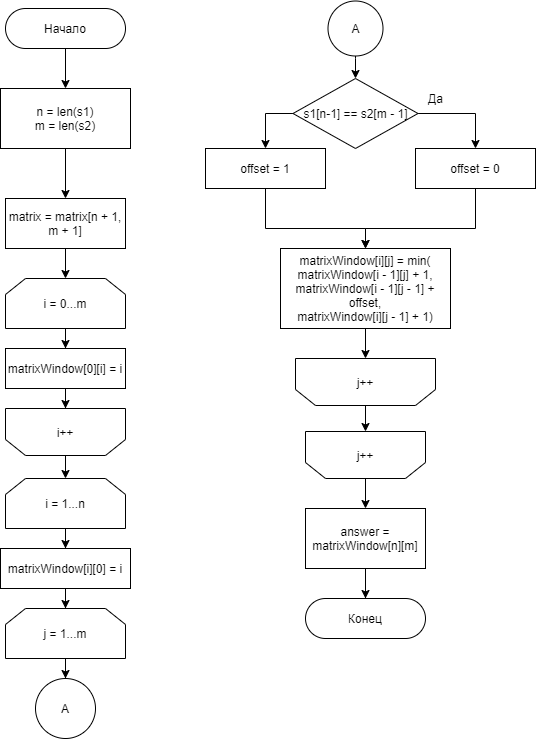
\includegraphics[scale=0.9]{LevenshtainMatrix}
		 	\caption{Матричный алгоритм поиска расстояния Левенштейна}
		 	\label{LevenshtainMatrix}
	 	\end{figure}
	 	\begin{figure}
		 	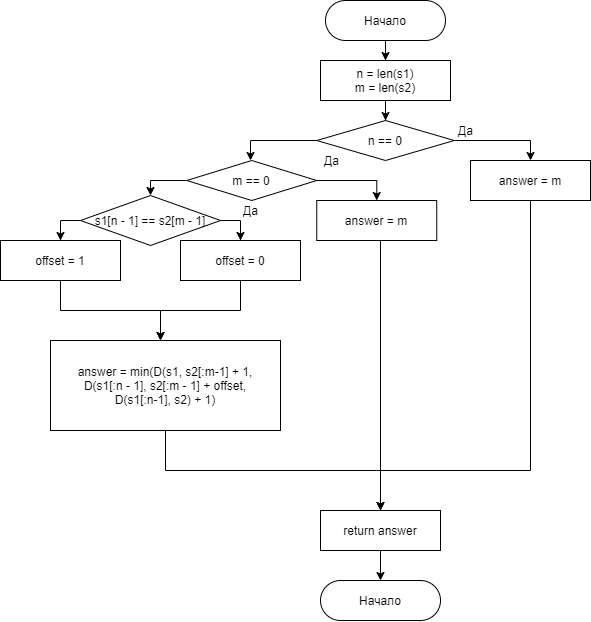
\includegraphics[scale=0.9]{LevenshtainRecursiveMatrixless}
		 	\caption{Рекурсивный алгоритм поиска расстояния Левенштейна без матрицы}
		 	\label{LevenshtainRecursiveMatrixless}
	 	\end{figure}
	 	\begin{figure}
	 		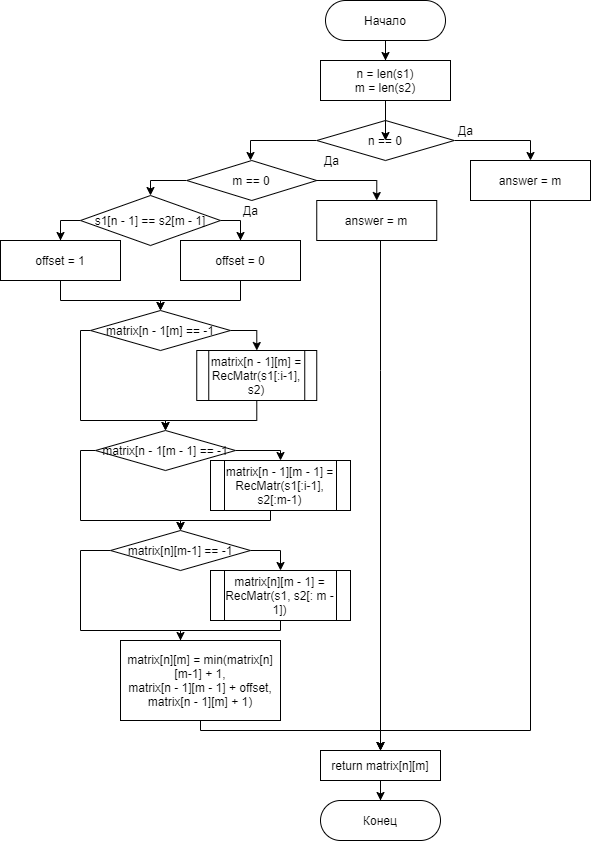
\includegraphics[scale=0.7]{LevenshtainRecursiveMatrix}
		 	\caption{Рекурсивный алгоритм поиска расстояния Левенштейна}
		 	\label{LevenshtainRecursiveMatrix}
	 	\end{figure}
	 	\begin{figure}
		 	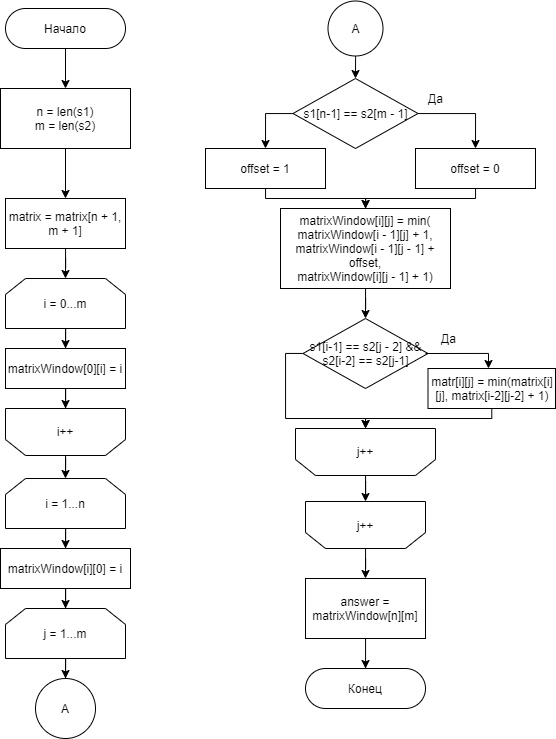
\includegraphics[scale=0.9]{DamerauLevenshtainMatrix}
		 	\caption{Матричный алгоритм поиска расстояния Дамерау-Левенштейна}
		 	\label{DamerauLevenshtainMatrix}
	 	\end{figure}
	 	\newpage
		 \subsection{Оценка затрачиваемой памяти}
		 При матричной реализации алгоритмов память занимает:
		 \begin{enumerate}
 		 	\item два входных слова длинами n и m;	
		 	\item матрица размером (n + 1)*(m + 1);
		 	\item две переменные, хранящие длины слов;
		 	\item четыре вспомагательные переменные. (i, j, answer, correction).
		 \end{enumerate}
	 	
	 	Таким образом размер занимаемой памяти составляет \ref{levenshtainMatrixCapacity}:
	 	\begin{equation}\label{levenshtainMatrixCapacity}
	 	C_{\text{общ}} = C_1 * ((n + 1) * (m + 1) + 2 + 4) + C_2 * (n + m)
	 	\end{equation}
	 	
	 	При рекурсивной реализации при каждом вызове требуется выделять 4 переменных размером $C_2$. Максимальная глубина рекурсии равна (n + m).
	 	Максимальный объем занимаемой памяти - \ref{levenshtainRecursiveCapacity}:
	 	\begin{equation}\label{levenshtainRecursiveCapacity}
	 	C_{\text{общ}} = (n + m) * (C_1 * 4 + C_2 * (n + m)) + C_1 * (n + 1) * (m + 1)
	 	\end{equation}
	\newpage
	\section{Технологическая часть}
	Ниже будут представлены средствы реализации и листинги реализованной программы.
	\subsection{Средcтва реализации}
	Выбранный язык программирования - Go, так как он структурный, в нем можно легко писать код, а требований по конкретнему языку не выдвигалось.\cite{vs-code} Среда разработки - Visual Studio Code.\cite{golang}
	\newline
	\indent Функция вычисления процессорного времени использует функцию QueryPerfomanceCounter из библиотеки WinAPI.\cite{winapi} Функция представлена на листинге 1.
	\newline
	\indent Листинг 1. Функция замера процессорного времени.
	\begin{lstlisting}
	func getProcessorTime() (int64) {
	dll, err := syscall.LoadDLL("kernel32.dll")
	if err != nil {
		fmt.Printf("Error 1")
		return 0;
	}
	qpc, err := dll.FindProc("QueryPerformanceCounter")
	if err != nil {
		fmt.Printf("Error 2")
		return 0;
	}
	var ctr int64
	ret, _, _ := qpc.Call(uintptr(unsafe.Pointer(&ctr)))
	if ret == 0 {
		return 0
	}
	return ctr
}
	\end{lstlisting}
	\subsection{Реализации алгоритмов}
	Ниже представлены листинги реализаций следующего алгоритма:
	\begin{itemize}
	\item листинг 2. Матричный алгоритм нахождения расстояния Левенштейна,
	\item листинг 3. Рекурсивный алгоритм нахождения расстояния Левенштейна без матрицы,
	\item листинг 4. Рекурсивный алгоритм нахождения расстояния Левенштейна с матрицей,
	\item листинг 5. Матричный алгоритм нахождения расстояния Дамерау-Левенштейна
	\end{itemize}
	Листинг 2. Реализация алгоритма поиска расстояния Левенштейна.
	\begin{lstlisting}
func LevenshtainMatrixNotWindow(s1, s2 []rune) (answer int) {
	firstLenght := len(s1)
	secondLenght := len(s2)
	if firstLenght == 0 && secondLenght > 0 {
		answer = secondLenght
	} else if secondLenght == 0 && firstLenght > 0 {
		answer = firstLenght
	} else {
		matrix := make([][]int, len(s1) + 1)
		for i := 0; i <= len(s1); i++ {
			matrix[i] = make([]int, len(s2) + 1)
		}
		for i := 0; i < secondLenght+1; i++ {
			matrix[0][i] = i
		}
		for i := 1; i < firstLenght+1; i++ {
			matrix[i][0] = i
			for j := 1; j < secondLenght+1; j++ {

				if matrix[i - 1][j] < matrix[i][j-1] {
					matrix[i][j] = matrix[i - 1][j]
				} else {
					matrix[i][j] = matrix[i][j-1]
				}
				matrix[i][j]++
				diagonalStep := matrix[i-1][j-1]
				if s1[i-1] != s2[j-1] {
					diagonalStep++
				}
				if diagonalStep < matrix[i][j] {
					matrix[i][j] = diagonalStep
				}
			}
		}
		answer = matrix[firstLenght][secondLenght]
	}
	return answer
}
	\end{lstlisting}
	
	Листинг 3. Реализация рекурсивного алгоритма поиска расстояния Левенштейна без матрицы.
	\begin{lstlisting}
	func LevenshtainRecursiveMatrixless(s1, s2 []rune) (answer int) {
	firstLenght := len(s1)
	secondLenght := len(s2)

	if firstLenght == 0 {
		answer = secondLenght
	} else if secondLenght == 0 {
		answer = firstLenght
	} else {
		lastSymbolFirst := s1[firstLenght - 1]
		lastSymbolSecond := s2[secondLenght - 1]
		
		correction := 1
		if (lastSymbolFirst == lastSymbolSecond) {
			correction = 0
		}
		s1 = s1[:firstLenght - 1]
		answer = LevenshtainRecursiveMatrixless(s1, s2) + 1
		s2 = s2[:secondLenght - 1]
		answerMiddle := LevenshtainRecursiveMatrixless(s1, s2) + correction
		s1 = append(s1, lastSymbolFirst)
		answerSecond := LevenshtainRecursiveMatrixless(s1, s2) + 1
		s1 = append(s2, lastSymbolSecond)

		if answerMiddle < answer {
			answer = answerMiddle
		}
		if answerSecond < answer {
			answer = answerSecond
		}
	}
	return answer
}
	\end{lstlisting}
	
		Листинг 4. Реализация рекурсивного алгоритма поиска расстояния Левенштейна с матрицей.
	\begin{lstlisting}
	func LevenshtainRecursiveMatrixBody(s1, s2 []rune, matrix [][]int) (answer int) {
	firstLenght := len(s1)
	secondLenght := len(s2)

	if firstLenght == 0 {
		answer = secondLenght
	} else if secondLenght == 0 {
		answer = firstLenght
	} else {
		lastSymbolFirst := s1[firstLenght - 1]
		lastSymbolSecond := s2[secondLenght - 1]
		
		correction := 1
		if (lastSymbolFirst == lastSymbolSecond) {
			correction = 0
		}
		s1 = s1[:firstLenght - 1]
		if (matrix[firstLenght - 1][secondLenght] == -1) {
			LevenshtainRecursiveMatrixBody(s1, s2, matrix)
		}
		answer = matrix[firstLenght - 1][secondLenght] + 1
		s2 = s2[:secondLenght - 1]
		if (matrix[firstLenght - 1][secondLenght - 1] == -1) {
			LevenshtainRecursiveMatrixBody(s1, s2, matrix)
		}
		answerMiddle := matrix[firstLenght - 1][secondLenght - 1] + correction
		s1 = append(s1, lastSymbolFirst)
		if (matrix[firstLenght][secondLenght - 1] == -1) {
			LevenshtainRecursiveMatrixBody(s1, s2, matrix)
		}
		answerSecond := matrix[firstLenght][secondLenght - 1] + 1
		s1 = append(s2, lastSymbolSecond)

		if answerMiddle < answer {
			answer = answerMiddle
		}
		if answerSecond < answer {
			answer = answerSecond
		}
	}
	matrix[firstLenght][secondLenght] = answer
	return answer
}
	\end{lstlisting}
		Листинг 5. Реализация матричного алгоритма поиска расстояния Дамерау-Левенштейна.
	\begin{lstlisting}
	func DamerauLevenshtainMatrix(s1, s2 []rune) (answer int) {
	firstLenght := len(s1)
	secondLenght := len(s2)
	if firstLenght == 0 && secondLenght > 0 {
		answer = secondLenght
	} else if secondLenght == 0 && firstLenght > 0 {
		answer = firstLenght
	} else {
		matrix := make([][]int, len(s1) + 1)
		for i := 0; i <= len(s1); i++ {
			matrix[i] = make([]int, len(s2) + 1)
		}

		for i := 0; i < secondLenght+1; i++ {
			matrix[0][i] = i
		}
		for i := 1; i < firstLenght+1; i++ {
			matrix[i][0] = i
			for j := 1; j < secondLenght+1; j++ {
				if matrix[i-1][j] < matrix[i-1][j-1] {
					matrix[i][j] = matrix[i-1][j]
				} else {
					matrix[i][j] = matrix[i][j-1]
				}
				matrix[i][j]++
				diagonalStep := matrix[i-1][j-1]
				if s1[i-1] != s2[j-1] {
					diagonalStep++
				}
				if diagonalStep < matrix[i][j] {
					matrix[i][j] = diagonalStep
				}
				
				if (i > 1 && j > 1 && s1[i - 1] == s2[j - 2] && s1[i - 2] == s2[j - 1]) {
					if (matrix[i - 2][j - 2] + 1 < matrix[i][j]) {
						matrix[i][j] = matrix[i - 2][j - 2] + 1
					}
				}
			}
		}
		answer = matrix[firstLenght][secondLenght]
	}
	return answer
}
	\end{lstlisting}
	
	\subsection{Тестирование}
	Тестирование осуществляется по принципу ``черного ящика''.
	Рассмотренные случаи:
	\begin{itemize}
	\item одна строка пустая, вторая нет;
	\item обе строки пустые;
	\item строки эквивалентны,
	\item строки состоят их одного символа;
	\item строки состоят из произвольного количества символов.
	\end{itemize}
	\newpage
	\section{Экспериментальная часть}
	В данной главе будут представлен пример работы программы, результат экспериментов по замеру времени и произведен сравнительный анализ алгоритмов по затрачиваемому времени.
	\subsection{Пример работы программы}
	Пример работы программы представлен на рисунке \ref{programmWork}
	 	\begin{figure}[h!]
		 	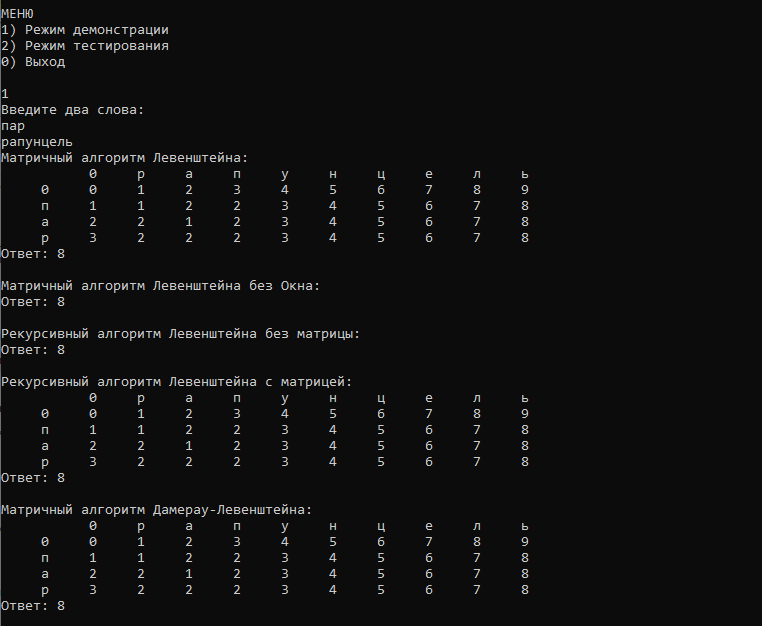
\includegraphics[scale=0.9]{programmWork}
		 	\caption{Пример работы программы со словами ``пар'' и ``рапунцель''}
		 	\label{programmWork}
	 	\end{figure}
	\subsection{Результаты тестирования}
	Результаты тестирования приведены в таблице \ref{testTable}.
	\newline
	\begin{table}
	\centering
		\caption{Результаты тестов} \label{testTable}
	\begin{tabular}{| c | c | c |}
	\hline
	Входные строки & Ожидаемое результат & Полученный результат \\ \hline
	`` `` & 0 & 0 \\ \hline
		`aba` `` & 3 & 3 \\ \hline
			`` `` & 0 & 0 \\ \hline
				`uwu` `uwu` & 0 & 0 \\ \hline
					`random` `rndm` & 2 & 2 \\ \hline
						`owl` `wolf` & 3/2 & 3/2 \\ \hline
	\end{tabular}
	\end{table}
	\subsection{Сравнительный анализ алгоритмов по времени}
	Эксперименты проводятся на строках длины от 1 до 10 с шагом 2 (результаты на рисунке \ref{smallTest})
		\begin{figure}[h!]
		 	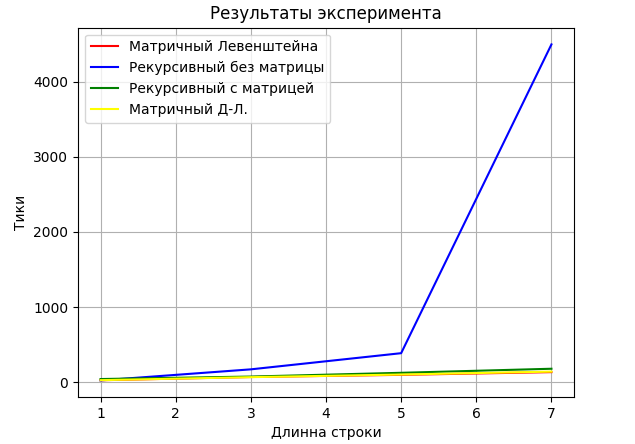
\includegraphics[scale=0.9]{smallTest}
		 	\caption{Замеры времени на строках малой длины}
		 	\label{smallTest}
	 	\end{figure}
	 	
	И на строках длины от 50 до 550 с шагом 100 (результаты на рисунке \ref{longTest})
	
	 	\begin{figure}[h!]
		 	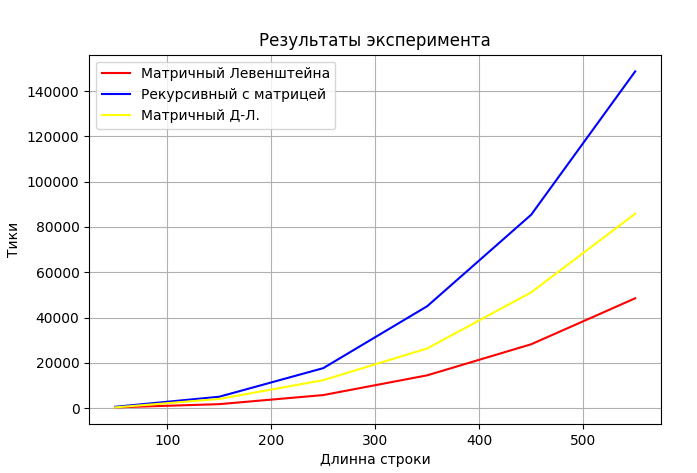
\includegraphics[scale=0.9]{longTest}
		 	\caption{Замеры времени на строках большой длины}
		 	\label{longTest}
	 	\end{figure}
	 	\newpage
	Как видно из графиков, самым долгим алгоритмом является рекурсивный алгоритм без использования матрицы. Самым быстрым является матричный алгоритм. Рекурсивный матричный алгоритм быстрее простого рекурсивного, но сильно уступает матричным реализациям.
		\newpage
	\begin{center}
		\section*{Заключение}
	\end{center}
	\addcontentsline{toc}{section}{Заключение}
	В этой лабораторной работе были изложены теоретические основы расстояний Левенштейна и Дамерау-Левенштейна, были разработаны и реализованы алгоритмы  мх поиска, проведены эксперименты по замеру времени работы разработанных алгоритмов и проведены сравнения алгоритмов по результатам эксперимента. Также была дана теоритическая оценка затрачиваемой памяти.
	\newpage
	\begin{center}
		\section*{Список литературы}
	\end{center}
	\addcontentsline{toc}{section}{Список литературы}
\begin{thebibliography}{2}
\bibitem{vs-code}
Visual Studio Code [Электронный ресурс]. Режим доступа: (дата обращения - 02.10.2020) Свободный. URL: code.visualstudio.com
\bibitem{golang}
Golang [Электронный ресурс]. Режим доступа: (дата обращения - 02.10.2020) Свободный. URL: http://golang-book.ru/
\bibitem{winapi}
WinAPI. Функция QueryPerformanceCounter [Электронный ресурс]. Режим доступа: (дата обращения - 02.10.2020) Свободный. URL: https://docs.microsoft.com/en-us/windows/win32/api/profileapi/nf-profileapi-queryperformancecounter
\end{thebibliography}
\end{document}